\documentclass{classrep}
\usepackage[utf8]{inputenc}
\usepackage{color}
\usepackage{enumitem}
\usepackage{graphicx}
\usepackage{amsmath}
\usepackage{float}
\usepackage{hyperref}

\studycycle{Informatyka, studia dzienne, I st.}
\coursesemester{VI}

\coursename{Komputerowe systemy rozpoznawania}
\courseyear{2019/2020}

\courseteacher{dr hab. inż. Adam Niewiadomski prof. uczelni}
\coursegroup{pon., 12:15}

\author{
\studentinfo{Mateusz Walczak}{216911} \and
\studentinfo{Konrad Kajszczak}{216790}
}

\title{Zadanie 2: Lingwistyczne podsumowania baz danych}
\svnurl{https://github.com/Walducha1908/KSR2}

\begin{document}
\maketitle

\section{Cel}
\textit{Praca w toku}


\section{Wprowadzenie}
\textit{Praca w toku}


\section{Opis implementacji}
\textit{Praca w toku}


\section{Materiały i metody}
Wybrana przez nas baza danych zawiera historyczne pomiary pogodowe z Holandii \cite{baza}. Dane zostały zgromadzone przez KNMI (\textit{Dutch weather institute} - Holenderski instytut pogodowy) na przestrzeni lat 1901-2018 i pochodziły z 50 różnych stacji pogowych znajdujących się na terenie całego kraju.\newline

Ze względu na fakt, iż oryginalna baza danych składa się z 804099 krotek, postanowiliśmy wybrać tylko niewielką część z dostępnych danych. Zdecydowaliśmy się na najnowsze dane pomiarowe - z lat 2016-2018. W ten sposób ograniczyliśmy liczbę wykorzystywanych krotek do 17000.\newline

\subsection{Wybór kolumn}
W celu analizy bazy danych i tworzenia jej lingwistycznych podsumowań wybraliśmy następujące 10 kolumn z danymi liczbowymi:

\begin{itemize}[label=$\bullet$\scshape\bfseries]
\item FG - średnia prędkość wiatru przez cały dzień [$0.1 \frac{m}{s}$].
\item FHX - najwyższa średnia prędkość wiatru w ciągu jednej godziny [$0.1 \frac{m}{s}$].
\item FHN - najniższa średnia prędkość wiatru w ciągu jednej godziny [$0.1 \frac{m}{s}$].
\item FXX - najszybszy podmuch wiatru w ciągu całego dnia [$0.1 \frac{m}{s}$].
\item TG - średnia dzienna temperatura [$0.1^{\circ} C$].
\item TN - minimalna dzienna temperatura [$0.1^{\circ} C$].
\item TX - maksymalna dzienna temperatura [$0.1^{\circ} C$].
\item T10N - minimalna dzienna temperatura na wysokości 10 cm od poziomu gruntu [$0.1^{\circ} C$].
\item Q - nasłonecznienie, energia słoneczna przypadająca na powierzchnię [$\frac{J}{cm^2}$].
\item RH - suma opadów atmosferycznych w ciągu całegi dnia [$0.1 mm$].\newline
\end{itemize}

Oprócz wyżej opisanych danych liczbowych, w naszej bazie znajdują się także dwie dodatkowe kolumny, służące do identyfikacji pomiaru:
\begin{itemize}[label=$\bullet$\scshape\bfseries]
\item STN - numer stacji badawczej wykonującej pomiar.
\item YYYYMMDD - data pomiaru w formacie opisanym przez nazwę kolumny.
\end{itemize}

\begin{figure}[H]
	\centering
	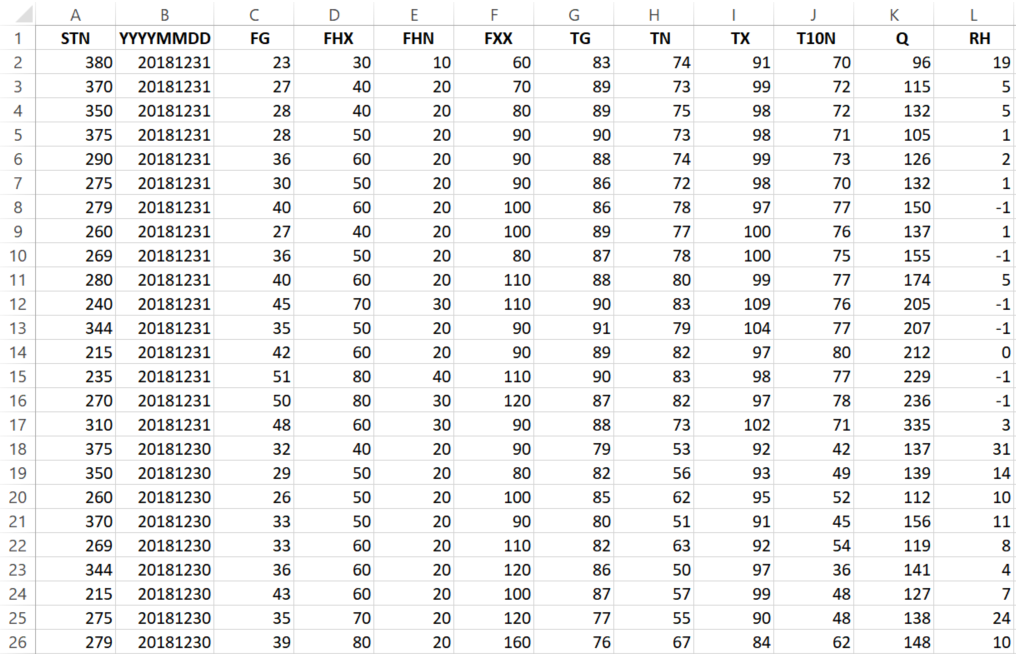
\includegraphics[width=1\textwidth]{Pictures/baza.png}
	\caption{Fragment widoku bazy w formacie $xlsx$}
\end{figure}

\subsection{Przykładowe zmienne lingwistyczne}
W poniższych tabelach zaproponowano przykładowe zmienne lingwistyczne dla wybranych atrybutów \footnote{Wartości prezentowane w tabelach są tylko propozycjami. Autorzy sprawozdania zastrzegają sobie możliwość do ich późniejszej modyfikacji}.

\begin{table}[H]
	\centering
	\begin{tabular}{c c c c c} 
		\hline
		\textbf{Etykieta} & \textbf{a} & \textbf{b} & \textbf{c} & \textbf{d}\\ [0.5ex] 
		\hline
		\hline 
Gentle	 & 5 & 10 & 21 & 26 \\
Moderate & 25 & 32 & 42 & 49 \\
Strong	 & 48 & 75 & 125 & 157 \\
		\hline
	\end{tabular}
	\caption{Przyporządkowane parametry funkcji trapezoidalnej dla kolumny FG.}
\end{table}

\begin{table}[H]
	\centering
	\begin{tabular}{c c c c c} 
		\hline
		\textbf{Etykieta} & \textbf{a} & \textbf{b} & \textbf{c} & \textbf{d}\\ [0.5ex] 
		\hline
		\hline 
Cold	 & -81 & -50 & 50 & 75 \\
Warm     & 74 & 100 & 175 & 200 \\
Hot	       & 199 & 225 & 275 & 306 \\
		\hline
	\end{tabular}
	\caption{Przyporządkowane parametry funkcji trapezoidalnej dla kolumny TG.}
\end{table}

\begin{table}[H]
	\centering
	\begin{tabular}{c c c c c} 
		\hline
		\textbf{Etykieta} & \textbf{a} & \textbf{b} & \textbf{c} & \textbf{d}\\ [0.5ex] 
		\hline
		\hline 
Overcast	  & 24 & 150 & 375 & 500 \\
Cloudy     & 499 & 700 & 1300 & 1500 \\
Sunny	  & 1499 & 1900 & 2700 & 3145 \\
		\hline
	\end{tabular}
	\caption{Przyporządkowane parametry funkcji trapezoidalnej dla kolumny Q.}
\end{table}






\section{Wyniki}
\textit{Praca w toku}


\section{Dyskusja}
\textit{Praca w toku}


\section{Wnioski}
\textit{Praca w toku}


\begin{thebibliography}{1}
\bibitem{baza} 
Baza danych - 
\href{https://www.kaggle.com/sinaasappel/historical-weather-in-the-netherlands-19012018}{\textit{"Historical weather in the Netherlands 1901-2018"}}
\end{thebibliography}
\end{document}
